\problemname{Bonsai}

Mange siger, at de dyrker bonsai, fordi det er »vanskeligt« eller »harmonisk«.
Det er nu ikke defor, Torstina gør det.
Hun vil bare score kassen på at sælge træerne, så hun får råd til at købe en masse jamaicaæbler.
Hun har lige sat en ny knold i jorden, mens hun drømme om næste jamaicaæble.
Hvor mange år skal hun mon vente til hun har det bonsaitræ, hendes kunde ønsker sig?

Bonsaitræer består af $2\leq N \leq 10^5$ knolde og $N-1$ grene.
Knuderne er nummereret fra $0$ til $N-1$. 
Alle bonsaitræer begynder med en lille knold, som man sætter ned i jorden.
Hvert år vokser der en ny gren ud fra hver knold, og i grenens ende dannes en ny knold.
Man kan klippe grene af træet når som helst. 
Torstina minder dig om, at det ikke spiller nogen rolle, hvor roden sidder i træet.

Givet kundens beskrivelse af træet, hvor mange år skal Torstina vente, inden hun har dyrket sådan et træ?

\section*{Indlæsning}

Første række indeholder et heltal $N\geq 2$, antallet af knolde i kundens ønskede bonsaitræ.
De følgende $N$ linjer beskriver bonsaitræet på følgende måde:
På linje $i$ står først et heltal $0 < m_i < n$, antallet af grene udgående fra den $i$te knold. 
Derefter folger $m_i$ heltal, som besriver knoldene, der sidder sammenn med den $i$te knold.

\section*{Udskrift}
Et heltal $A$, antallet af år det tager Torstina at fremavle det bonsaitræ, som kunden beskriver.

\section*{Pointsætning}

Din løsning bliver testet på en mængde af testfaldsgrupper.
For at få point for en gruppe, skal du klare alle test i gruppen. 

\noindent
\begin{tabular}{| l | l | l |}
\hline
Gruppe & Pointværdi & Begrænsninger \\ \hline
1     & 14         &  $m_i\leq 2$.\\ \hline
2     & 26         &  $N \leq 100$. \\ \hline
3     & 30         &  $m_i \leq 3$. \\ \hline
4     & 15          &  $A \leq 15$. \\ \hline
5     & 15          &  Ingen yderligere begrænsninger. \\ \hline
\end{tabular}

\section*{Forklaring af eksempelfald 1}
Torstina kan fremavle træet på to år ved at lade det vokse som i nedenstående figur.

\begin{figure}[h]
	\centering
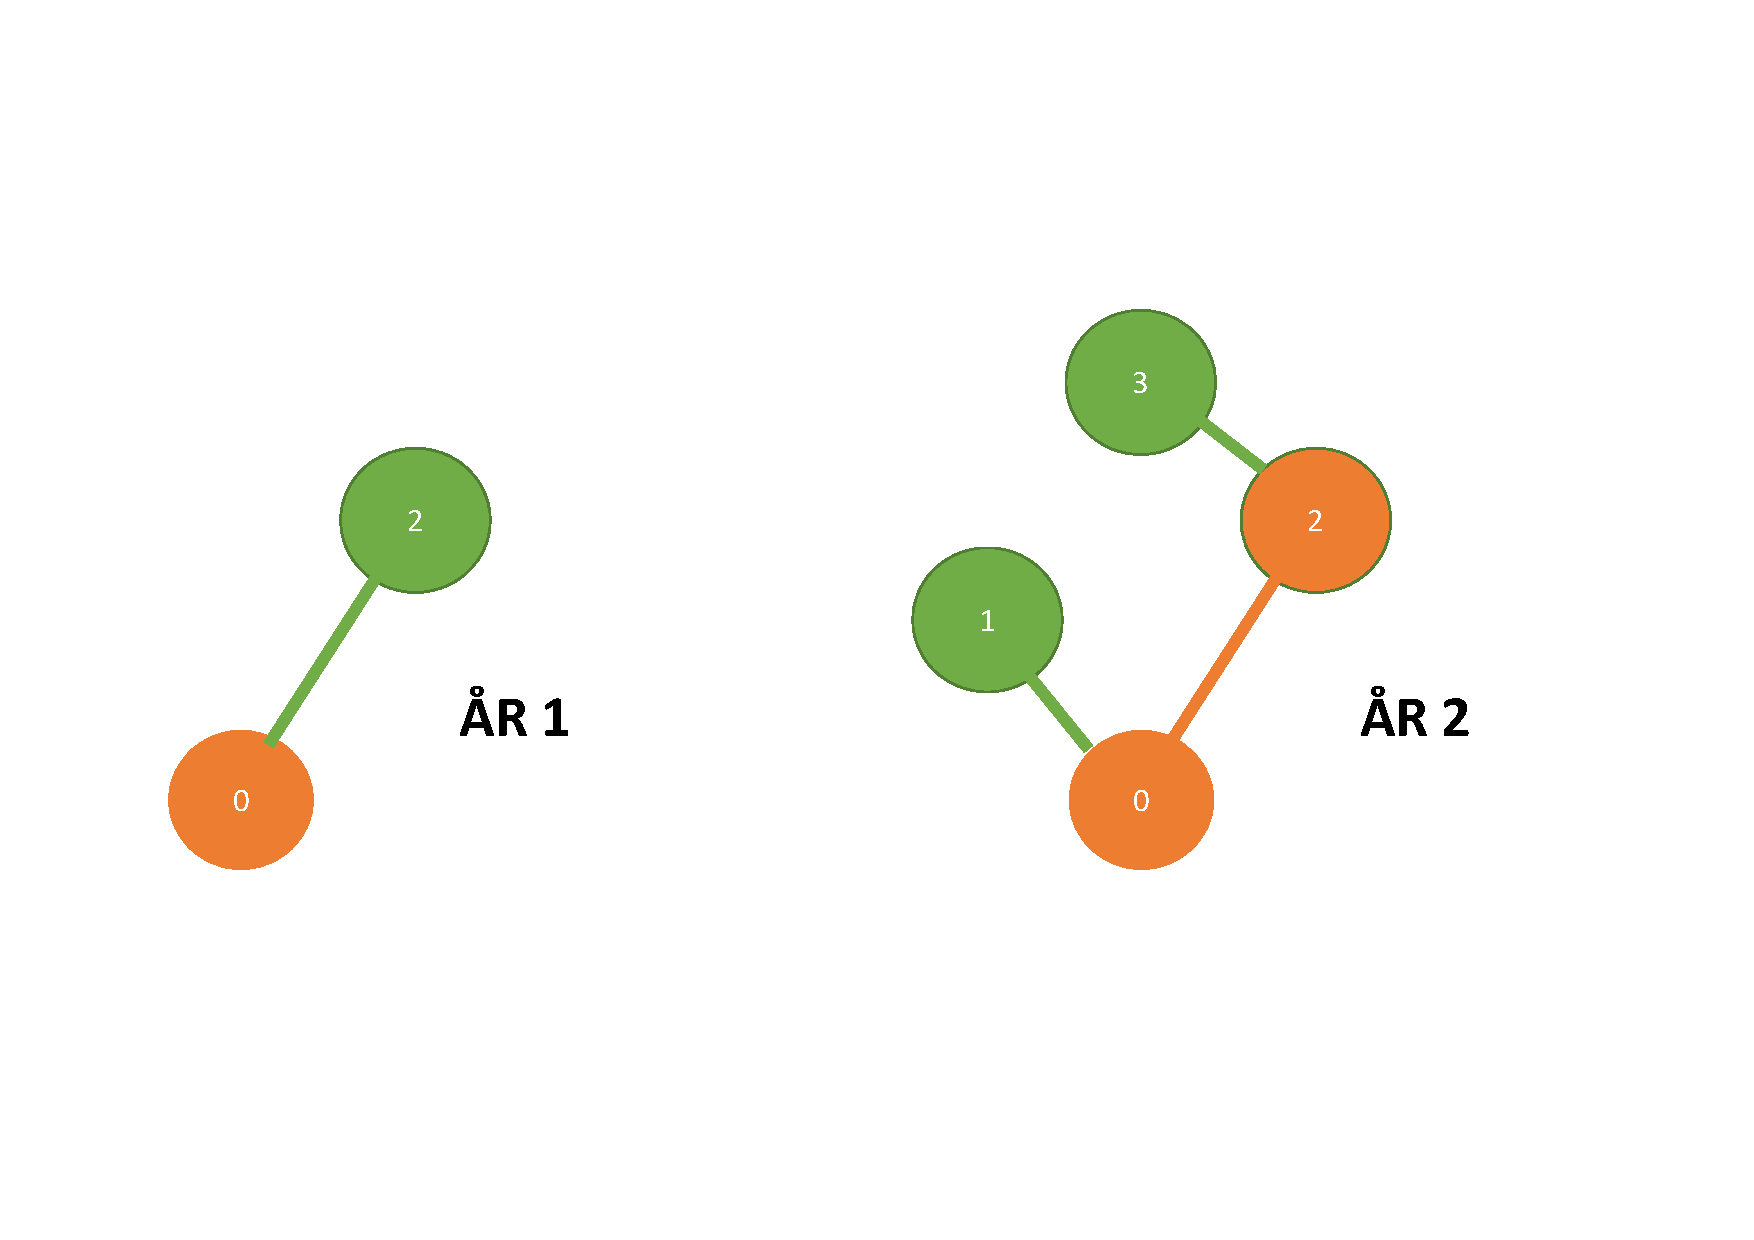
\includegraphics[width=0.5\textwidth]{Bonsai_tree}
\caption{En af de to måder man kan fremavle bonsaitræet i eksempel  1 på to år.}
\end{figure}
